\documentclass[11pt]{article}
\usepackage[margin=1in]{geometry}
\usepackage{amsmath,amssymb,amsthm,mathtools}
\usepackage{tikz,tikz-cd}
\usepackage{amsmath,amssymb}
\usetikzlibrary{arrows.meta,decorations.markings,backgrounds,cd,calc}
\colorlet{c1}{blue!70!black}\colorlet{c2}{red!70!black}\colorlet{c3}{green!45!black}
\tikzset{
 ->-/.style={decoration={markings,mark=at position .55 with {\arrow{Stealth[length=2.4mm]}}},postaction={decorate}},
 ->>-/.style={decoration={markings,mark=at position .5 with {\arrow{Stealth[length=2.4mm]}},mark=at position .6 with {\arrow{Stealth[length=2.4mm]}}},postaction={decorate}},
 every picture/.append style={show background rectangle, background rectangle/.style={fill=white}}
}

\usepackage{enumitem}
\usepackage[most]{tcolorbox}
\usepackage[colorlinks=true,linkcolor=blue!60!black]{hyperref}

\newcommand{\Z}{\mathbb Z}
\newcommand{\R}{\mathbb R}
\newcommand{\RP}{\mathbb{RP}}
\newcommand{\Hred}{\tilde H}
\newcommand{\im}{\operatorname{im}}
\newcommand{\coker}{\operatorname{coker}}
\newtcolorbox{note}{colback=gray!6,colframe=gray!60,boxrule=0.5pt,arc=2pt}
\newtcolorbox{exambox}{colback=white,colframe=black,boxrule=0.5pt,arc=0pt}
\setlength{\parindent}{0pt}\setlength{\parskip}{4pt}
\emergencystretch=3em

\newcommand{\prob}[2]{\par\medskip\textbf{#1.} \textit{(#2 points)}\ }

\title{MATH730 Midterm II --- extra practice}
\date{}
\begin{document}
\maketitle
\vspace{-2.5em}

There are two mock exams in the style of the practice midterm: 3 problems, 10 points each, 50 minutes. Try each one under exam conditions, with no notes. After them are three extra problems. Solutions are in the appendix.

%=====================================================
\section*{Mock exam A}
\begin{exambox}
\prob{1}{10} Let $X$ be the space obtained from $S^2$ by identifying two distinct points. Find a $\Delta$-complex structure on $X$ and use it to compute the simplicial homology of $X$.

\prob{2}{10}
\begin{enumerate}[label=(\alph*),leftmargin=*]
\item \textit{(4 points)} Define a $\Delta$-complex.
\item \textit{(6 points)} Define the boundary map $\partial_n:C_n(X)\to C_{n-1}(X)$ on singular chains, and prove that $\partial_{n-1}\circ\partial_n=0$.
\end{enumerate}

\prob{3}{10} Let $X\subseteq\R^3$ be the union of the unit sphere $S^2$ and the equatorial disk $D=\{(x,y,0):x^2+y^2\le1\}$. Use the Mayer--Vietoris sequence to compute $H_k(X)$ for all $k$.
\end{exambox}

%=====================================================
\section*{Mock exam B}
\begin{exambox}
\prob{1}{10} Let $X$ be the space obtained by attaching a 2-cell to $S^1$ along the map $S^1\to S^1$, $z\mapsto z^3$. In other words, $X$ is a disk whose boundary circle is wrapped three times around a circle. Find a $\Delta$-complex structure on $X$ and use it to compute the simplicial homology of $X$.

\prob{2}{10}
\begin{enumerate}[label=(\alph*),leftmargin=*]
\item \textit{(3 points)} For $A\subseteq X$, define the relative chain complex $C_\bullet(X,A)$ and the relative homology groups $H_n(X,A)$.
\item \textit{(3 points)} State the long exact sequence of the pair $(X,A)$, and describe the connecting map $H_n(X,A)\to H_{n-1}(A)$ explicitly.
\item \textit{(4 points)} Show that if two chain maps $f,g:C_\bullet\to D_\bullet$ are chain homotopic, then $f_*=g_*:H_n(C)\to H_n(D)$ for all $n$.
\end{enumerate}

\prob{3}{10} Let $A\subseteq X$ and suppose $r:X\to A$ is a retraction, i.e.\ $r\circ i=\mathrm{id}_A$ where $i:A\hookrightarrow X$ is the inclusion.
\begin{enumerate}[label=(\alph*),leftmargin=*]
\item \textit{(7 points)} Use the long exact sequence of the pair $(X,A)$ to show that $H_n(X)\cong H_n(A)\oplus H_n(X,A)$ for every $n$.
\item \textit{(3 points)} Deduce that $S^{n-1}$ is not a retract of $D^n$ for any $n\ge1$.
\end{enumerate}
\end{exambox}

%=====================================================
\section*{Extra problems}
\begin{enumerate}[label=\textbf{E\arabic*.},leftmargin=*]
\item Let $M$ be the Möbius band and $\partial M\cong S^1$ its boundary circle. You may use that $M$ deformation retracts onto its core circle, and that the inclusion $\partial M\hookrightarrow M$ induces multiplication by $2$ on $H_1\cong\Z$.
\begin{enumerate}[label=(\alph*)]
\item Use the long exact sequence of the pair to compute $H_k(M,\partial M)$ for all $k$.
\item $(M,\partial M)$ is a good pair, and $M/\partial M\cong\RP^2$. Explain why your answer is consistent with $H_*(\RP^2)$.
\end{enumerate}
\item Let $X\subseteq\R^3$ be the union of $S^2$ and the segment joining the north and south poles. Use Mayer--Vietoris to compute $H_*(X)$. Compare with Mock exam A, Problem 1.
\item Let $T^2$ be the torus, and $A\cong S^1\vee S^1$ the image of the boundary of the square (the 1-skeleton).
\begin{enumerate}[label=(\alph*)]
\item Compute $H_*(T^2,A)$. (Hint: good pairs.)
\item Using (a) and the long exact sequence of the pair, show that the inclusion induces an isomorphism $H_1(A)\to H_1(T^2)$. You may use $H_1(T^2)\cong\Z^2$ and $H_2(T^2)\cong\Z$.
\end{enumerate}
\end{enumerate}

%=====================================================
\clearpage
\appendix
\section*{Appendix: solutions}

%-----------------------------------------------------
\subsection*{Mock A, Problem 1: $S^2$ with two points identified}

\textbf{Reduction.} For $n\ge2$, any two pairs of distinct points of $S^n$ can be exchanged by a homeomorphism of $S^n$. So the space does not depend on which two points we identify, and we may take them to be vertices of a $\Delta$-complex structure on $S^2$.

\textbf{Structure.} Take the usual structure on $S^2$: two 2-simplices $U$ and $L$ glued along their entire boundaries. Each has vertices $v_0,v_1,v_2$, and the shared edges are $a=[v_0,v_1]$, $b=[v_1,v_2]$, $c=[v_0,v_2]$. Now identify $v_0$ with $v_2$, and call the result $v$; set $w=v_1$.
\begin{center}
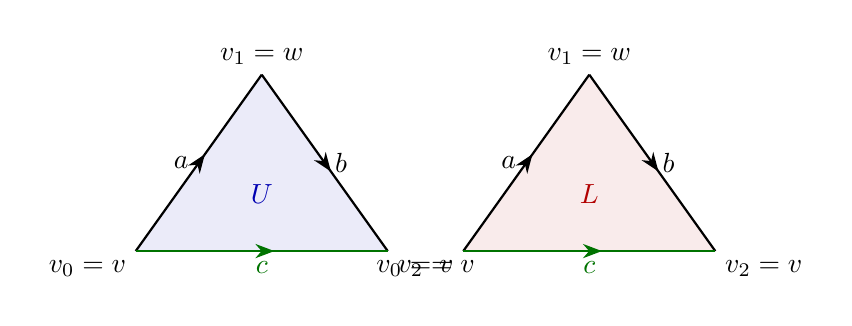
\begin{tikzpicture}[scale=1.6]
\foreach \s/\n/\col in {0/U/c1,2.6/L/c2}{
\begin{scope}[xshift=\s cm]
\coordinate (A) at (0,0); \coordinate (B) at (1,1.4); \coordinate (C) at (2,0);
\fill[\col!8] (A)--(B)--(C)--cycle;
\draw[thick,->-] (A)--node[left]{$a$}(B);
\draw[thick,->-] (B)--node[right]{$b$}(C);
\draw[thick,c3,->-] (A)--node[below]{$c$}(C);
\node[below left] at (A){$v_0=v$}; \node[above] at (B){$v_1=w$}; \node[below right] at (C){$v_2=v$};
\node[\col] at (1,0.45){$\n$};
\end{scope}}
\end{tikzpicture}
\end{center}
This is still a $\Delta$-complex: identifying two vertices is allowed (a simplex's vertices need not be distinct in $X$), and the edge orders are unchanged. Now $c$ is a loop at $v$.

\textbf{Boundaries.}
\[\partial U=\partial L=b-c+a,\qquad\partial a=w-v,\quad\partial b=v-w,\quad\partial c=0.\]

\textbf{Homology.}
\begin{itemize}
\item $H_0$: $\im\partial_1=\langle w-v\rangle$, so $H_0=\Z^2/\langle w-v\rangle\cong\Z$.
\item $H_1$: $\partial_1(xa+yb+zc)=(x-y)(w-v)$, so $\ker\partial_1=\{x=y\}$ has basis $\{a+b,\ c\}$. The image $\im\partial_2=\langle a+b-c\rangle$ is $(1,-1)$ in this basis, which is primitive (part of the basis $\{(1,-1),(0,1)\}$). So $H_1\cong\Z^2/\langle(1,-1)\rangle\cong\Z$, generated by $[c]$.
\item $H_2$: $\partial_2(pU+qL)=(p+q)(a+b-c)$, so $\ker\partial_2=\langle U-L\rangle\cong\Z$. There are no 3-simplices, so $H_2\cong\Z$.
\end{itemize}
\[\boxed{H_0=\Z,\quad H_1=\Z,\quad H_2=\Z,\quad H_k=0\ (k\ge3).}\]
\begin{note}
Sanity check: $X\simeq S^2\vee S^1$. Slide one of the two points along an arc until they touch, and the arc becomes a loop. The new loop $c$ is exactly the image of the edge joining the two identified points.
\end{note}

%-----------------------------------------------------
\subsection*{Mock A, Problem 2}

\textbf{(a)} A $\Delta$-complex structure on a space $X$ is a collection of maps $\sigma_\alpha:\Delta^{n_\alpha}\to X$ such that:
\begin{enumerate}[label=(\roman*)]
\item each restriction $\sigma_\alpha|_{\operatorname{int}\Delta^{n_\alpha}}$ is injective, and every point of $X$ lies in the image of exactly one such restriction;
\item each restriction of $\sigma_\alpha$ to a face is one of the maps $\sigma_\beta$, i.e.\ $\sigma_\alpha\circ\iota_i=\sigma_\beta$ for some $\beta$, where $\iota_i:\Delta^{n-1}\to\Delta^n$ is the $i$-th face inclusion (preserving vertex order);
\item $U\subseteq X$ is open if and only if $\sigma_\alpha^{-1}(U)$ is open in $\Delta^{n_\alpha}$ for every $\alpha$.
\end{enumerate}

\textbf{(b)} $C_n(X)$ is the free abelian group on all continuous maps $\sigma:\Delta^n\to X$. On generators,
\[\partial_n\sigma=\sum_{i=0}^n(-1)^i\,\sigma|_{[v_0,\dots,\hat v_i,\dots,v_n]},\]
extended linearly. Here $\sigma|_{[v_0,\dots,\hat v_i,\dots,v_n]}=\sigma\circ\iota_i$ is regarded as a singular $(n-1)$-simplex via the order-preserving identification with $\Delta^{n-1}$.

\emph{Proof that $\partial\partial=0$.} It suffices to check on a generator $\sigma$. Applying $\partial$ twice, and splitting according to whether the second deleted vertex $v_j$ comes before or after the first deleted vertex $v_i$:
\[\partial\partial\sigma=\sum_{j<i}(-1)^i(-1)^j\,\sigma|_{[\dots,\hat v_j,\dots,\hat v_i,\dots]}+\sum_{j>i}(-1)^i(-1)^{j-1}\,\sigma|_{[\dots,\hat v_i,\dots,\hat v_j,\dots]}.\]
In the second sum, $v_j$ is in position $j-1$ once $v_i$ has been deleted, which gives the sign $(-1)^{j-1}$. Swapping the names $i$ and $j$ turns the second sum into
\[\sum_{i>j}(-1)^j(-1)^{i-1}\,\sigma|_{[\dots,\hat v_j,\dots,\hat v_i,\dots]}=-\sum_{j<i}(-1)^{i+j}\,\sigma|_{[\dots,\hat v_j,\dots,\hat v_i,\dots]},\]
which cancels the first sum. Hence $\partial\partial\sigma=0$. \qed

(In words: each codimension-2 face, missing $v_j$ and $v_i$, appears twice, once for each order of deleting the two vertices, and with opposite signs.)

%-----------------------------------------------------
\subsection*{Mock A, Problem 3: sphere with an equatorial disk}

Let $0$ be the center of $D$ and $E=\partial D$ the equator.
\begin{itemize}
\item $A=X\setminus\{0\}$ is open, and it deformation retracts onto $S^2$: push $D\setminus\{0\}$ radially out onto $E$, fixing $S^2$. So $A\simeq S^2$.
\item $B=D\cup\{p\in S^2:|z(p)|<\tfrac12\}$, the disk together with an open band around the equator. It is open, since its complement in $X$ is the closed set $\{p\in S^2:|z(p)|\ge\tfrac12\}$. It deformation retracts onto $D$ by sliding the band along meridians onto $E$, so it is contractible.
\item $A\cap B=(D\setminus\{0\})\cup\text{band}$. It deformation retracts onto $E\cong S^1$: push the band to $E$ and the punctured disk radially out to $E$. So $A\cap B\simeq S^1$.
\end{itemize}
$A\cup B=X$ and $A\cap B\neq\emptyset$, so reduced MV applies:
\[\Hred_k(A\cap B)\to\Hred_k(A)\oplus\Hred_k(B)\to\Hred_k(X)\to\Hred_{k-1}(A\cap B)\to\Hred_{k-1}(A)\oplus\Hred_{k-1}(B).\]
\begin{itemize}
\item $k=2$: $\ \Hred_2(S^1)=0\to\Hred_2(S^2)\oplus0=\Z\to\Hred_2(X)\to\Hred_1(S^1)=\Z\to\Hred_1(S^2)\oplus0=0$. This gives a short exact sequence $0\to\Z\to H_2(X)\to\Z\to0$. Since $\Z$ is free, it splits, so $H_2(X)\cong\Z^2$.
\item $k=1$: $\ \Hred_1(S^1)=\Z\to0\to\Hred_1(X)\to\Hred_0(S^1)=0$, so $H_1(X)=0$.
\item $k\ge3$: $\ 0\to\Hred_k(X)\to\Hred_{k-1}(S^1)=0$, so $H_k(X)=0$.
\item $k=0$: $X$ is path-connected, so $H_0(X)=\Z$.
\end{itemize}
\[\boxed{H_0=\Z,\quad H_1=0,\quad H_2=\Z^2,\quad H_k=0\ (k\ge3).}\]
\begin{note}
Sanity check: the disk cuts the sphere into two hemispheres, each closed up by $D$, so you see two 2-spheres sharing the disk. Collapsing the contractible $D$ gives $X\simeq S^2\vee S^2$.
\end{note}

%-----------------------------------------------------
\subsection*{Mock B, Problem 1: the disk wrapped three times}

\textbf{Structure.} Model $X$ as a triangle $p_0p_1p_2$ whose three boundary edges are all identified with one loop $a$, all oriented the same way around ($p_0\to p_1\to p_2\to p_0$). Going around the boundary then reads $aaa$, i.e.\ the boundary wraps three times. A single triangle cannot carry these orientations (the arrows around it would form a cycle), so add a center vertex $c$ and cone off:
\begin{center}
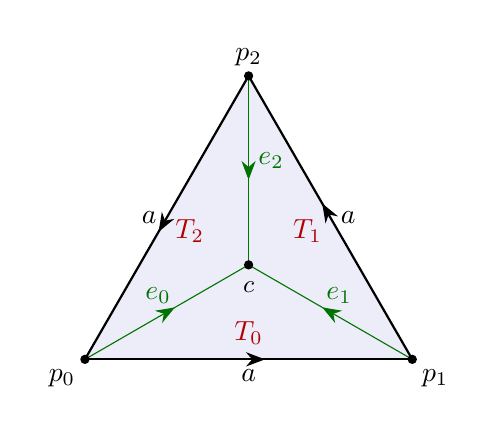
\begin{tikzpicture}[scale=2.4]
\coordinate (P0) at (210:1); \coordinate (P1) at (330:1); \coordinate (P2) at (90:1); \coordinate (C) at (0,0);
\fill[c1!7] (P0)--(P1)--(P2)--cycle;
\draw[thick,->-] (P0)--node[below]{$a$}(P1);
\draw[thick,->-] (P1)--node[right]{$a$}(P2);
\draw[thick,->-] (P2)--node[left]{$a$}(P0);
\draw[c3,->-] (P0)--node[above left=-2pt,pos=0.55]{$e_0$}(C);
\draw[c3,->-] (P1)--node[above right=-2pt,pos=0.55]{$e_1$}(C);
\draw[c3,->-] (P2)--node[right,pos=0.45]{$e_2$}(C);
\node[below left] at (P0){$p_0$}; \node[below right] at (P1){$p_1$}; \node[above] at (P2){$p_2$}; \node[font=\small] at (-90:0.12){$c$};
\node[c2] at (270:0.36){$T_0$}; \node[c2] at (30:0.36){$T_1$}; \node[c2] at (150:0.36){$T_2$};
\foreach \p in {P0,P1,P2,C} \fill (\p) circle(0.7pt);
\end{tikzpicture}
\end{center}
\begin{itemize}
\item Vertices: $v=p_0=p_1=p_2$ and $c$.
\item Edges: the loop $a$, and the spokes $e_i=[p_i,c]$.
\item 2-simplices: $T_i=[p_i,p_{i+1},c]$ (indices mod 3), with $[p_i,p_{i+1}]=a$.
\end{itemize}
Every edge's orientation matches the vertex order in each triangle, so this is a $\Delta$-complex.

\textbf{Boundaries.}
\[\partial T_i=e_{i+1}-e_i+a,\qquad\partial a=0,\qquad\partial e_i=c-v.\]

\textbf{Homology.}
\begin{itemize}
\item $H_0$: $\im\partial_1=\langle c-v\rangle$, so $H_0\cong\Z$.
\item $H_2$: $\partial_2(\sum n_iT_i)=\sum_i(n_{i-1}-n_i)e_i+(n_0+n_1+n_2)a$. This is $0$ only if all $n_i$ are equal, say to $n$, and $3n=0$; so $n=0$. Hence $H_2=0$.
\item $H_1$: $\partial_1(xa+\sum y_ie_i)=(\sum y_i)(c-v)$, so $\ker\partial_1$ has basis $a,\ f_1=e_1-e_0,\ f_2=e_2-e_1$. The boundaries are
\[\partial T_0=a+f_1,\qquad\partial T_1=a+f_2,\qquad\partial T_2=a-f_1-f_2.\]
In the quotient, the first two relations give $f_1=-a$ and $f_2=-a$. Substituting into the third gives $3a=0$. So $H_1$ is generated by $[a]$ subject only to $3[a]=0$, and $H_1\cong\Z/3$. (Check: the relation matrix has determinant $\pm3$.)
\end{itemize}
\[\boxed{H_0=\Z,\quad H_1=\Z/3,\quad H_2=0.}\]
\begin{note}
This matches the cell-attachment picture from the review: $\varphi_*:H_1(S^1)\to H_1(S^1)$ is multiplication by $3$. It is injective, so there is no new $H_2$, and $H_1=\coker(\times3)=\Z/3$.
\end{note}

%-----------------------------------------------------
\subsection*{Mock B, Problem 2}

\textbf{(a)} $C_n(A)$ is a subcomplex of $C_n(X)$, since $\partial$ maps chains in $A$ to chains in $A$. Define $C_n(X,A)=C_n(X)/C_n(A)$, with the boundary map induced by $\partial$. This is well defined because $\partial(C_n(A))\subseteq C_{n-1}(A)$, and it still satisfies $\partial\partial=0$. Then $H_n(X,A)=H_n(C_\bullet(X,A))$. Concretely:
\begin{itemize}
\item a relative cycle is a chain $z\in C_n(X)$ with $\partial z\in C_{n-1}(A)$;
\item it is a relative boundary if $z=\partial w+a$ with $w\in C_{n+1}(X)$ and $a\in C_n(A)$.
\end{itemize}

\textbf{(b)} The LES of the pair is
\[\cdots\to H_n(A)\xrightarrow{i_*}H_n(X)\xrightarrow{j_*}H_n(X,A)\xrightarrow{d}H_{n-1}(A)\xrightarrow{i_*}H_{n-1}(X)\to\cdots\to H_0(X,A)\to0.\]
Here $i$ is the inclusion and $j$ the quotient map. The connecting map is $d[z]=[\partial z]$: represent the class by a relative cycle $z$; then $\partial z$ is a cycle in $A$. This is the general recipe applied to $0\to C(A)\to C(X)\to C(X,A)\to0$: lift $z$ to $C(X)$ (it already is a chain there), take its boundary, and observe that it lies in $C(A)$.

\textbf{(c)} Let $P$ be a chain homotopy, so $\partial P+P\partial=g-f$. If $z\in C_n$ is a cycle, then
\[g(z)-f(z)=\partial P(z)+P(\partial z)=\partial P(z),\]
which is a boundary. So $[g(z)]=[f(z)]$ in $H_n(D)$, i.e.\ $g_*[z]=f_*[z]$. \qed

%-----------------------------------------------------
\subsection*{Mock B, Problem 3: retracts}

\textbf{(a)} By functoriality, $r_*i_*=(r\circ i)_*=\mathrm{id}$, so $i_*:H_n(A)\to H_n(X)$ is injective for every $n$. Now look at the LES:
\[H_n(A)\xrightarrow{i_*}H_n(X)\xrightarrow{j_*}H_n(X,A)\xrightarrow{d}H_{n-1}(A)\xrightarrow{i_*}H_{n-1}(X).\]
\begin{itemize}
\item Exactness at $H_{n-1}(A)$: $\im d=\ker i_*=0$, so $d=0$.
\item Exactness at $H_n(X,A)$: $\im j_*=\ker d=H_n(X,A)$, so $j_*$ is surjective.
\end{itemize}
So $0\to H_n(A)\xrightarrow{i_*}H_n(X)\xrightarrow{j_*}H_n(X,A)\to0$ is short exact. It splits, because $r_*$ is a left inverse of $i_*$. Explicitly, $\Phi:H_n(X)\to H_n(A)\oplus H_n(X,A)$, $\Phi(x)=(r_*x,\,j_*x)$, is an isomorphism:
\begin{itemize}
\item \emph{Injective:} if $r_*x=0$ and $j_*x=0$, then $x=i_*a$ for some $a$ (exactness), and $a=r_*i_*a=r_*x=0$.
\item \emph{Surjective:} given $(a,y)$, pick $x'$ with $j_*x'=y$ and set $x=x'+i_*(a-r_*x')$. Then $j_*x=y$ (since $j_*i_*=0$), and $r_*x=r_*x'+a-r_*x'=a$.
\end{itemize}

\textbf{(b)} If $S^{n-1}$ were a retract of $D^n$, then by (a) $H_{n-1}(S^{n-1})$ would be isomorphic to a subgroup (a direct summand) of $H_{n-1}(D^n)$.
\begin{itemize}
\item For $n\ge2$: $H_{n-1}(S^{n-1})=\Z$ but $H_{n-1}(D^n)=0$.
\item For $n=1$: $H_0(S^0)=\Z^2$ but $H_0(D^1)=\Z$, and $\Z^2$ is not isomorphic to a subgroup of $\Z$.
\end{itemize}
Either way we get a contradiction. \qed

%-----------------------------------------------------
\subsection*{E1: the Möbius band relative to its boundary}

\textbf{(a)} $H_*(M)\cong H_*(S^1)$ and $H_*(\partial M)\cong H_*(S^1)$. The LES of the pair:
\begin{align*}
&\underbrace{H_2(M)}_0\to H_2(M,\partial M)\to\underbrace{H_1(\partial M)}_{\Z}\xrightarrow{\times2}\underbrace{H_1(M)}_{\Z}\to\\
&\qquad\to H_1(M,\partial M)\to\underbrace{H_0(\partial M)}_{\Z}\xrightarrow{\cong}\underbrace{H_0(M)}_{\Z}\to H_0(M,\partial M)\to0.
\end{align*}
\begin{itemize}
\item $H_0(\partial M)\to H_0(M)$ is an isomorphism, since both spaces are path-connected and a point generates each. So $H_0(M,\partial M)=0$.
\item Since that map is injective, $H_1(M,\partial M)\to H_0(\partial M)$ is zero. So $H_1(M,\partial M)\cong\coker(\times2)=\Z/2$.
\item $\times2$ is injective, so $H_2(M,\partial M)=0$.
\item For $k\ge3$, everything around $H_k(M,\partial M)$ vanishes.
\end{itemize}
\[H_0(M,\partial M)=0,\quad H_1(M,\partial M)=\Z/2,\quad H_k(M,\partial M)=0\text{ otherwise.}\]

\textbf{(b)} For a good pair, $H_k(M,\partial M)\cong\Hred_k(M/\partial M)=\Hred_k(\RP^2)$. This gives $\Hred_0=0$, $\Hred_1=\Z/2$, $\Hred_2=0$, which agrees with the practice midterm's Problem 1.

%-----------------------------------------------------
\subsection*{E2: sphere with a diameter}

Let $m$ be the midpoint of the segment.
\begin{itemize}
\item $A=X\setminus\{m\}$ deformation retracts onto $S^2$ by shrinking each half-segment to its pole. So $A\simeq S^2$.
\item $B$ is the segment together with two small open caps around the poles. It is open, and it deformation retracts onto the segment, so it is contractible.
\item $A\cap B=B\setminus\{m\}$ has two components, each contractible. So $A\cap B\simeq S^0$, with $\Hred_0=\Z$ and all other reduced groups $0$.
\end{itemize}
Reduced MV:
\begin{itemize}
\item $k=2$: $0\to\Hred_2(S^2)=\Z\to\Hred_2(X)\to\Hred_1(A\cap B)=0$, so $H_2(X)=\Z$.
\item $k=1$: $0\to\Hred_1(X)\to\Hred_0(A\cap B)=\Z\to\Hred_0(A)\oplus\Hred_0(B)=0$, so $H_1(X)=\Z$.
\item $k=0$: $H_0(X)=\Z$; and $H_k(X)=0$ for $k\ge3$.
\end{itemize}
This is the same answer as Mock A, Problem 1, and indeed $X\simeq S^2\vee S^1$ as well: contracting the segment to a point gives $S^2$ with the two poles identified.

%-----------------------------------------------------
\subsection*{E3: the torus relative to its 1-skeleton}

\textbf{(a)} $(T^2,A)$ is a good pair: $T^2$ minus a point of the open 2-cell is a neighborhood of $A$ that deformation retracts onto $A$. Collapsing the whole boundary of the square to a point gives $T^2/A\cong D^2/\partial D^2\cong S^2$. So
\[H_k(T^2,A)\cong\Hred_k(S^2)=\begin{cases}\Z&k=2,\\0&\text{otherwise.}\end{cases}\]

\textbf{(b)} The relevant part of the LES is
\[H_1(A)\xrightarrow{i_*}H_1(T^2)\to H_1(T^2,A)=0,\]
so $i_*:\Z^2\to\Z^2$ is surjective. A surjective homomorphism $\Z^2\to\Z^2$ is an isomorphism: its kernel $K$ satisfies $\Z^2/K\cong\Z^2$, and comparing ranks gives $\operatorname{rank}K=0$, so $K=0$ since $\Z^2$ is torsion-free. Hence $i_*$ is an isomorphism. (Also, $H_2(T^2)\to H_2(T^2,A)$ is an isomorphism $\Z\to\Z$, since $H_2(A)=0$ and $H_1(A)\to H_1(T^2)$ is injective.)

\end{document}
